\graphicspath{ {./figures/ratio/} }

%%%%%%%%%%%%%%%%%%%%%%%%%%%%%%%%%%%

\section{Supplementary figures}

\begin{figure}[h]
\centering
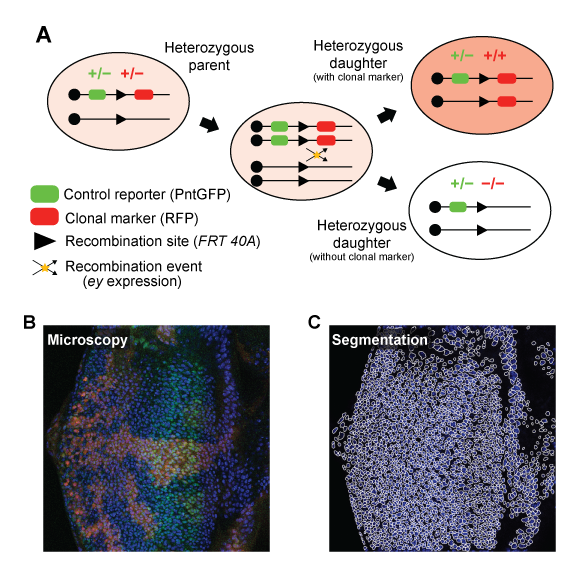
\includegraphics[width=1.0\columnwidth]{./figure_S1}
\caption[PntGFP expression during eye development.]{\textbf{PntGFP expression during eye development.} (A,B) Adult eyes of flies carrying (A) one or (B) two copies of the recombineered \textit{pnt-gfp} transgene under a \textit{pnt} null mutant background. Note the wildtype retina patterning under both rescue conditions. (C) Maximum intensity projections of Pnt-GFP fluorescence across layers spanning multipotent cells, differentiating R cells, and differentiating cones. White arrow denotes morphogenetic furrow. Black bars denote first and second periods of elevated Pnt-GFP expression. (D) Simultaneous Pnt-GFP (green) and Yan (magenta) expression dynamics in progenitor cells. Lines are smoothed moving averages across 500 sequential progenitors, shaded regions are bootstrapped 95\% confidence intervals for the mean. Arrows indicate the times at which local maxima occur.}
\label{fig:ratio:figS1}
\end{figure}

\begin{figure}[h]
\centering
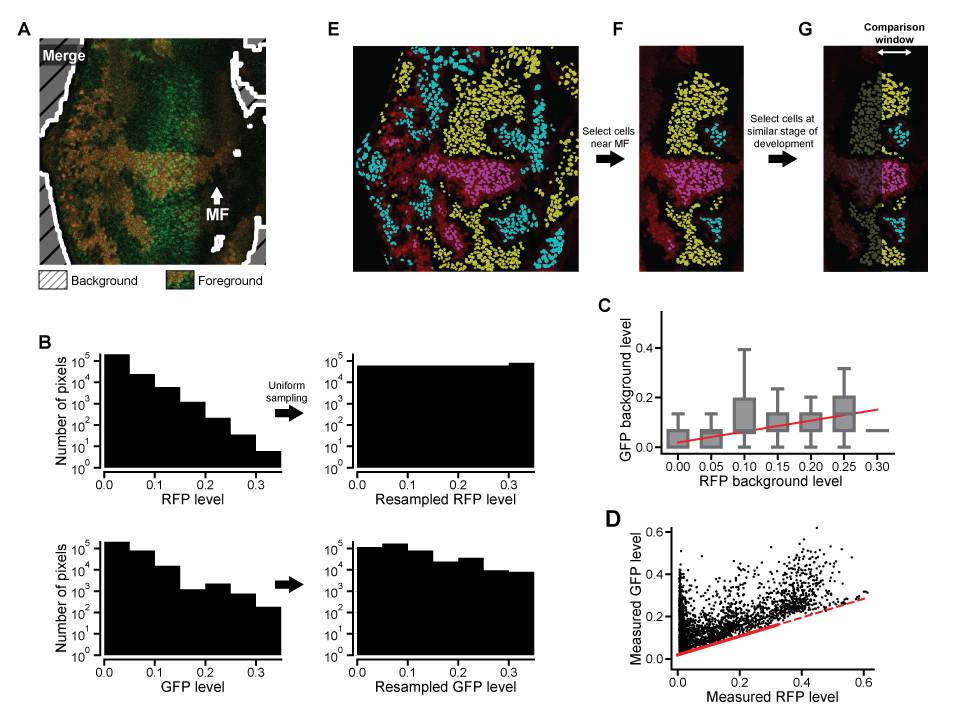
\includegraphics[width=1.0\columnwidth]{./figure_S2}
\caption[PntGFP and Yan expression dynamics in additional cell types.]{\textbf{PntGFP and Yan expression dynamics in additional differentiated cell types.} (A,B) Measured expression dynamics for all annotated cell types. Solid lines are moving averages across 250 and 75 sequential cells for progenitors and differentiating cells, respectively. Shading denotes bootstrapped 95\% confidence interval for the moving average. Colors denote cell type. (C-E) Expression dynamics and joint Pnt-Yan distributions for differentiating R8, R3/R4, and R7 cells. Joint distributions are limited to progenitor and R cells drawn from the shaded yellow region spanning the first ten R cells of the specified type in each disc. Solid lines are smoothed moving averages across 250 and 50 samples for progenitor and R cells, respectively. (F-G) Expression dynamics and joint Pnt-Yan distributions for differentiating C1/C2 and C3/C4 cone cells.}
\label{fig:ratio:figS2}
\end{figure}

%\begin{figure}[h]
%\centering
%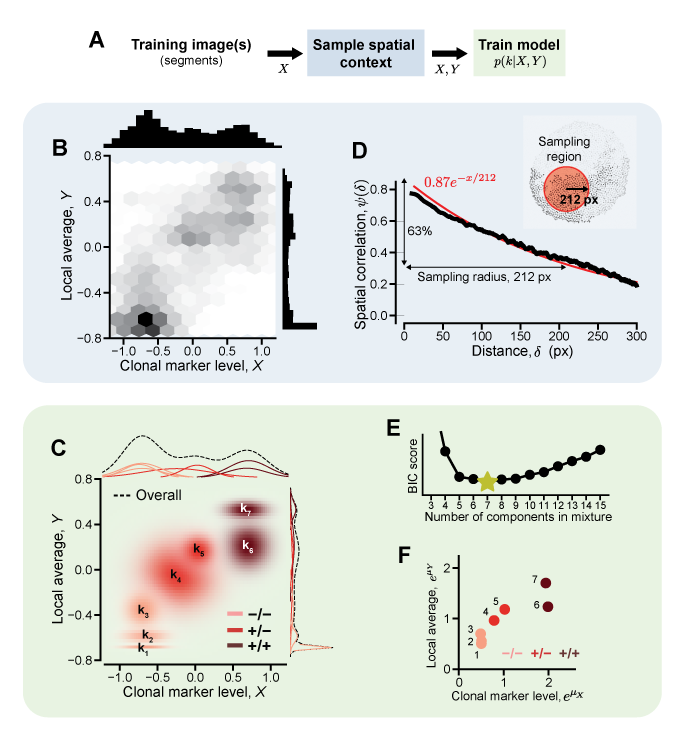
\includegraphics[width=1.0\columnwidth]{./figure_S3}
%\caption[Dynamics of expression variability in progenitors and R cells.]{\textbf{Dynamics of expression variability in progenitor and R8, R2/R5 and R1/R6 cells.} Heterogeneities of (A) Pnt expression, (B) Yan expression, and (C) the $log_2$-transformed ratio are estimated by de-trending fluctuations about a moving average of 250 sequential cells. Lines are moving averages of 250 sequential fluctuations, shaded regions are bootstrapped 95\% confidence intervals for the moving average. Colors denote cell type.}
%\label{fig:ratio:figS3}
%\end{figure}
%
%\begin{figure}[h]
%\centering
%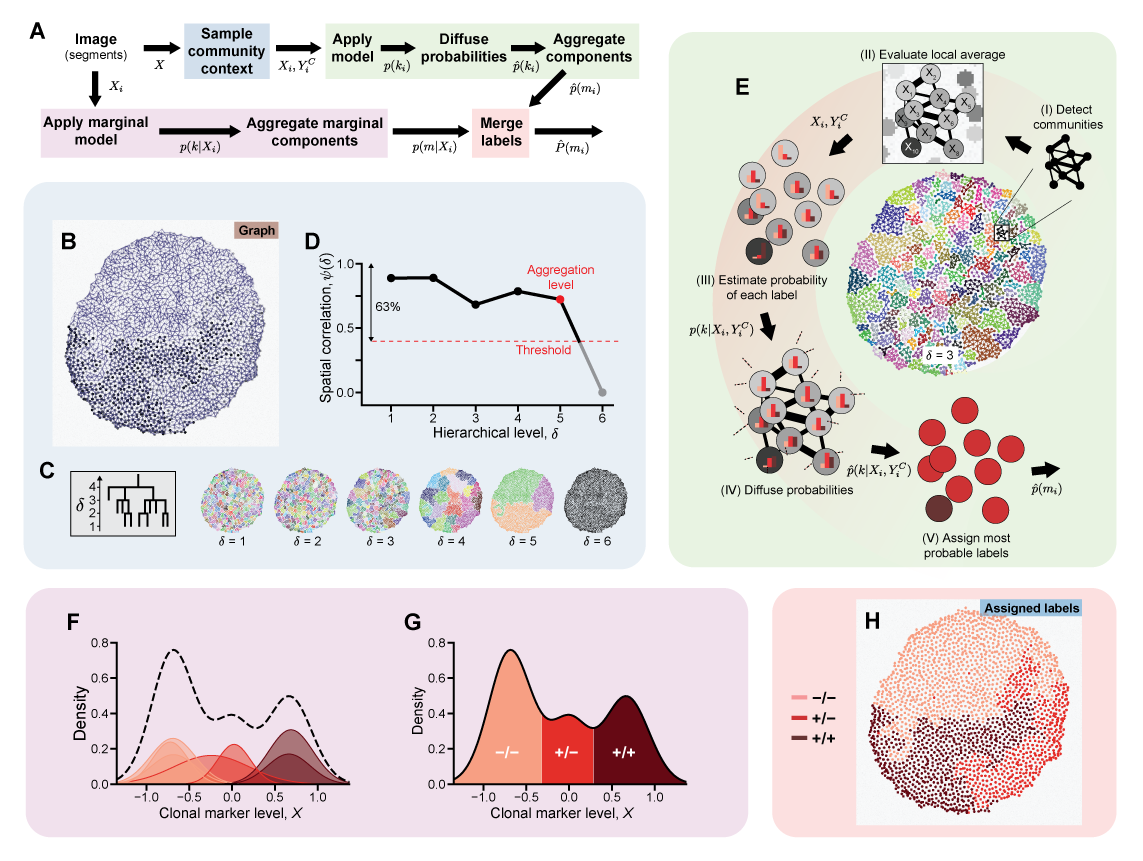
\includegraphics[scale=1.0]{./figure_S4}
%\caption[Simple two-species competitive binding model]{\textbf{A simple two-species competitive binding model} (A) Model schematic. (B) Theoretical Pnt site occupancy as a function of transcription factor abundance. Equivalent binding affinities are used for illustrative purposes. Simultaneous proportional increases in absolute abundance of both species have minimal impact on Pnt occupancy, while varying ratio confers maximal change.}
%\label{fig:ratio:figS4}
%\end{figure}
%
%\begin{figure}[h]
%\centering
%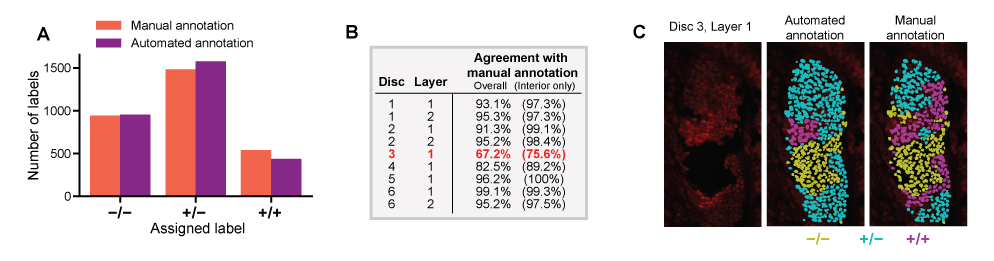
\includegraphics[width=0.9\columnwidth]{./figure_S5}
%\caption[Thermodynamic model of transcription factor DNA binding.]{\textbf{Thermodynamic model of transcription factor DNA binding.} (A) Summary of thermodynamic interactions within one microstate of a cis-regulatory element containing one ETS site and two non-ETS sites. Solid black lines represent individual binding sites. Green and magenta rectangles denote Pnt and Yan molecules. Example thermodynamic potentials of strong ETS-binding, weak non-ETS binding, and polymerization interactions are denoted by $\alpha_{Pnt}$, $\beta_{Yan}$, and $\gamma_{Yan}$, respectively. For this microstate, $a_P(k)=1$ and $a_Y(k)=2$. (B) Enumeration of all possible microstates for a cis-regulatory element of length 3 in which only the first site carries the ETS designation. Solid black lines denote binding sites, green and magenta rectangles denote bound Pnt and Yan molecules. The cumulative thermodynamic potentials of each microstate, $\Delta G_k$, are listed beside each graphical depiction. Visual representation is adapted from \cite{Hope2017}. (C) Relative thermodynamic contributions of binding site affinity versus polymerization to microstate statistical frequencies as a function of Pnt and Yan concentration. For each point in the plane, influence of site affinity was calculated by weighting the sum of all ETS and non-ETS thermodynamic potentials for each microstate by the statistical frequency of the corresponding microstate. The influence of polymerization was analogously determined. The shown color scale reflects the relative magnitude of these two summations, normalized by limits of zero and complete polymerization.}
%\label{fig:ratio:figS5}
%\end{figure}

\begin{figure}[h]
\centering
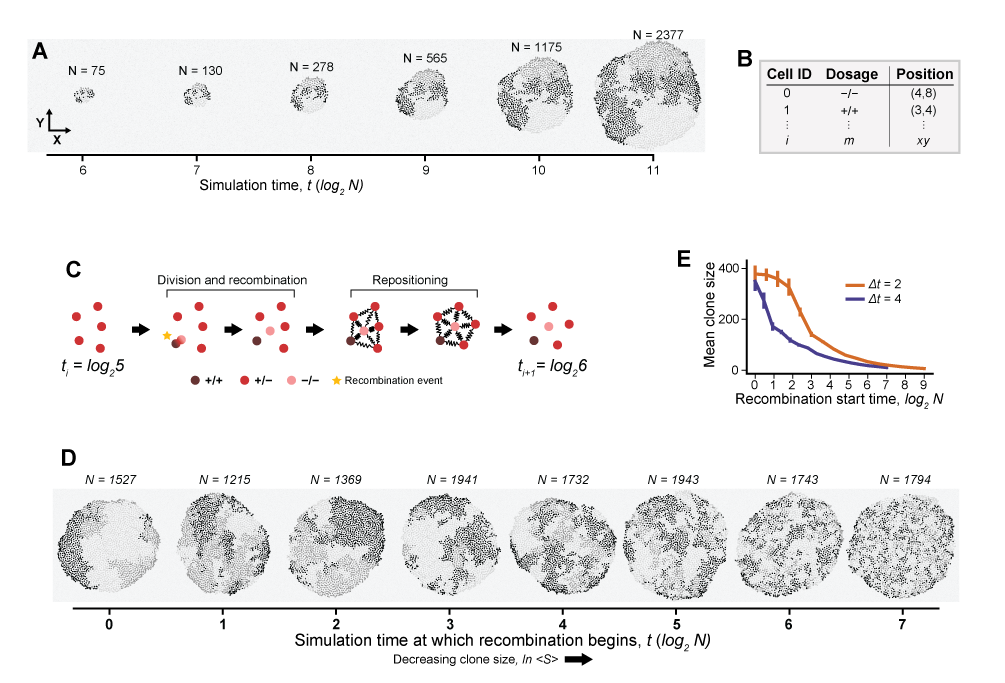
\includegraphics[width=1.0\columnwidth]{./figure_S6}
\caption[\textit{yan} null clones in the eye.]{\textbf{\textit{yan} null clones in the eye.} (A, B) Confocal images of (A) progenitor cells and (B) photoreceptors and cone cells in \textit{yan} null and heterozygote clones. Regions of Ubi-mRFPnls expression are manually labeled by \textit{yan} genotype. White text indicates regions of reduced Yan abundance, red denotes wildtype. DAPI visualizes all nuclei.}
\label{fig:ratio:figS6}
\end{figure}

\begin{figure}[h]
\centering
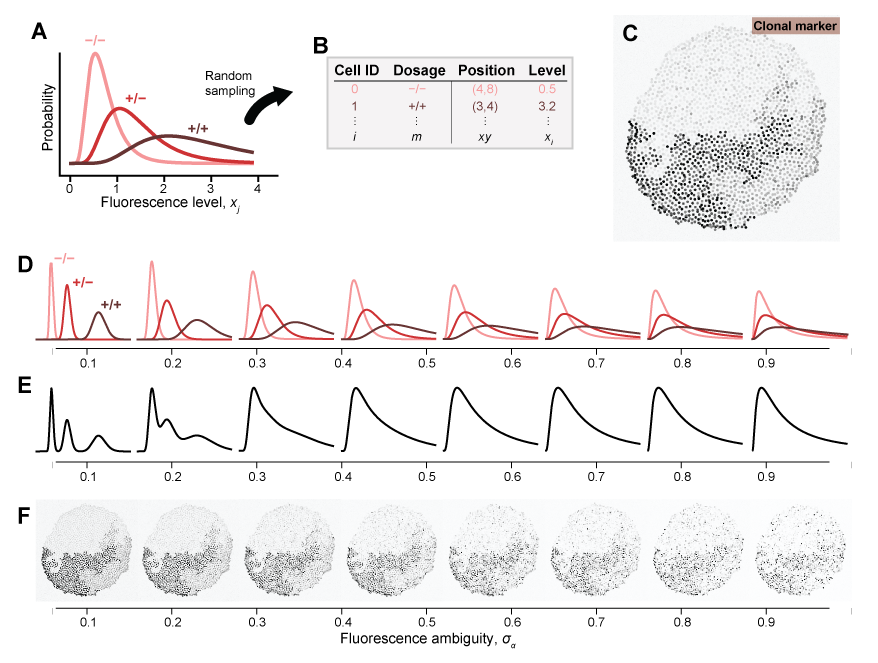
\includegraphics[width=1.0\columnwidth]{./figure_S7}
\caption[Spatial analysis of Pnt and Yan expression in $N^{ts}$ eye discs.]{\textbf{Spatial analysis of Pnt and Yan expression in $N^{ts}$ eye discs.} (A,B) Maximum intensity projections across confocal layers spanning progenitor cells when Notch signaling is (A) active and (B) restricted. Middle and right panels show Pnt-GFP and Yan expression, left panel shows merge in which Pnt-GFP is green and Yan is magenta. Black bars denote first and second periods of elevated Pnt-GFP expression. Dashed yellow line indicates crop boundary used to construct Figures \ref{fig:ratio:fig5}A and \ref{fig:ratio:fig5}B. (C,D) Distances between adjacent ommatidial columns in Notch mutant discs. (C) Procedure used to estimate inter-column distance. Neighboring R8 cells are identified by Delaunay triangulation, with an added constraint that edges must fall within 30 to 60 degrees of the anterior-posterior axis. The inter-column distance is estimated by averaging the anterior-posterior distance between neighbors (solid orange line). (D) Inter-column distances are more variable when Notch signaling is restricted (red) than under wildtype (grey) conditions. Black bars denote median, numbers above violins indicate the number of neighboring R8 cells. High variability prevents accurate estimation of MF velocity and precludes conversion of spatial positions to developmental times.}
\label{fig:ratio:figS7}
\end{figure}

%\begin{figure}[h]
%\centering
%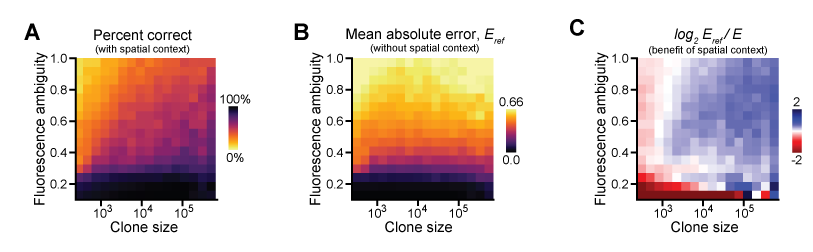
\includegraphics[width=1.0\columnwidth]{./figure_S8}
%\caption[Pnt and Yan expression dynamics in $EGFR^{ts}$ eye discs.]{\textbf{Pnt and Yan expression dynamics in $EGFR^{ts}$ eye discs.} (A-C) Effects of $EGFR^{ts}$ on (A) Pnt-GFP, (B) Yan, and (C) Pnt-to-Yan ratio dynamics in progenitor cells. Lines are moving averages across 250 sequential cells. Shaded regions are bootstrapped 95\% confidence intervals for the mean. Solid lines and grey shading denote wildtype controls. Dashed lines and red shading denote restricted EGFR signaling. Black bars denote second period of elevated Pnt-GFP expression.}
%\label{fig:ratio:figS8}
%\end{figure}
